%! TeX program = lualatex
\documentclass[
	english,
	accentcolor=9c,% Farbe für Hervorhebungen auf Basis der Deklarationen in den Corporate Design Richtlinien
  marginpar=0cm % TODO: Set this to 0 once todonotes is no longer needed
%	logofile=example-image, %Falls die Logo Dateien nicht vorliegen
	]{tudapub}

\usepackage{environ}
\usepackage{ifthen}
\newboolean{finalmode}
\setboolean{finalmode}{false}
\usepackage{float}

\usepackage[english]{babel}
\usepackage[autostyle]{csquotes}
\usepackage{xspace}
\usepackage[inline]{enumitem}
\usepackage{float}
\usepackage{listings}
\usepackage{booktabs}

\usepackage{mathtools}
\usepackage{amssymb}
\usepackage{bm}

\ifthenelse{\boolean{finalmode}}%
  {\usepackage[final]{microtype}}%
  {\usepackage[draft]{microtype}}%

\usepackage{cleveref}

\usepackage{todonotes}
\let\origtodo\todo
\RenewDocumentCommand{\todo}{o m}%
  {%
    \ifthenelse{\boolean{finalmode}}%
      {}%
      {%
        \IfNoValueTF{#1}%
          {\origtodo{#2}}%
          {\origtodo[#1]{#2}}%
      }%
  }%

% Wikipedia-style "citation needed" macro
% https://gist.github.com/martinarroyo/b9e0a963ad27169a6eee#gistcomment-2355734
\newcommand{\citeneeded}{%
  \ifthenelse{\boolean{finalmode}}%
    {}%
    {\textsuperscript{\color{blue} [citation needed]}\xspace}%
}

\usepackage{biblatex}
\bibliography{bibliography}

\usepackage{hologo}

\begin{document}

%Zusätzliche Metadaten für PDF/A. In diesem Fall notwendig, weil Titel ein Makro enthält.
\Metadata{
	author=Anton W. Haubner,
	title=Proposal: Masterthesis,
	subject=TBA,
	date=2021-10-21,
	keywords=TU Darmstadt \sep SE Group
}

\date{2021-10-21}
\title{Master Thesis Proposal}
\subtitle{Thesis Title (WIP!): Inspecting Java Program States with Semantic Web Technologies}
\author{Anton W. Haubner}

\titleimage{
%	%Folgende Box kann selbstverständlich durch ein mit \includegraphics geladenes Bild ersetzt werden.
	\color{black!30}\rule{\width}{\height}
}

\maketitle

%\begin{abstract}
%  % Criteria for a good abstract
%  % TOOD
%  \todo[inline]{TODO. But is an abstract really required?}
%\end{abstract}

\section{Motivation}

When implementing a concept from an application domain in a mainstream
programming language, its implementation may often differ strongly from its
original design.
This can be due to optimizations for efficiency because the implementation
language lacks the necessary expressiveness or due to other reasons.

For example, Simple Graphs are an abstract structure frequently used to model
and solve problems from many application domains.
E.g. they can be used to model computer networks, molecules from chemistry, etc.
%
They consist of vertices that are connected via edges.
However, to increase space-efficiency or performance of certain computations,
their representation in computer programs usually does not reflect this concept
directly.
Instead, they can for example be implemented as adjacency matrices where the
indices of a matrix model the vertices, while the matrix values indicate the
presence of an edge.
This representation may be preferred since it is space-efficient for non-sparse
graphs, it can look up in constant time whether two vertices are adjacent, and
one can directly apply methods of algebraic graph theory to it.

As such an implementation can differ so strongly from the original concept,
this complicates traditional debugging methods.
For instance, reviewing the adjacency matrix of a large graph in the value
inspector of a debugger does not reveal much insight into the structure.
%
Furthermore, optimized implementations like the adjacency matrix can often
syntactically represent structures that are invalid in the application domain.
Here, self-loops that connect vertices to themselves are not
allowed for Simple Graphs but can be represented by adjacency matrices with
entries on the diagonal.
Detecting such faulty structures during debugging is tedious or requires writing
custom code for analysis.

This problem intensifies if we move to even richer application domains.
For illustration, more complex types of graphs can be used to model molecules,
and graph rewriting systems can be utilized to explore their
reactions~\cite{yadav2004potential,mann2013graph}.
%
Debugging if and when a rewriting system implementation produces invalid or
unlikely molecules becomes tedious quickly due to the reasons listed above.

Instead, we can imagine a debugger that understands the application domain.
That is, it understands that atoms are modeled as vertices in a molecule graph
and that they have bond relations which each other. 
%
It also understands how these vertices are implemented in the terms of the
underlying programming language and what objects represent them in a program's
memory.

A debugger with this understanding of the application domain would allow us to
perform queries about complex concepts on the state of a program.
E.g. we could query \enquote{for all carbon atoms with more than four bonds}
which is a highly unlikely reaction result and could indicate a bug in the graph
rewriting system.
The debugger then could supply us with all adjacency matrix indices
corresponding to such atoms.

\paragraph{Semantic Debugging}

In \cite{kamburjan2021programming}, \citeauthor{kamburjan2021programming}
explore such ideas. They apply existing technologies of the Semantic
Web~\cite{semanticweb} to extract semantic knowledge databases from program
states. They formalized a minimal object-oriented language, \emph{SMOL}, and
extract knowledge in the well-supported RDF graph format.
%
This enables the application of semantic technology for analysis and debugging
of program states and even verification of programs.

For example, \citeauthor{kamburjan2021programming} introduce the idea of
\emph{Semantic Debugging}.
That is, a debugger that allows investigating program states without having to
manually inspect the call stack and heap memory.
Instead, the user can perform queries across the whole state using the
well-established SPARQL query language.
Furthermore, users may use the OWL language to define their own ontologies for
their application domain. This permits them to query the program state using
domain knowledge.

\Citeauthor{kamburjan2021programming} also demonstrate other uses of the
extracted RDF knowledge base.
E.g. invariants that reference concepts from the application domain which can be
proven using facts from the knowledge base.
They also demonstrate, how a knowledge base may be queried at runtime to give
programming languages reflection capabilities on the application domain level.

%% Implemented applications
% * State-access across whole stack
% * Semantic Debugging
%   * user-defined application domain
%   * Querying state for debugging (Answering Engine)
%   * Special Characteristics
%     * queries allow investigating large states without manually traversing
%       the call stack and heap memory
%     * ability to query using domain knowledge
%
% * Verification
%   * the generated knowledge base is FO-definable
%   * as are description logic formulae referencing domain knowledge.
%     This can be formulae like class invariants interesting in verification
%     contexts
%   * thus existing proof systems for FO invariants can make use of the
%     facts in the knowledge base as preconditions to proof such formulae
%
% * adding reflection capabilities to programming languages on the application
%   domain level
%
%%

% * using semantic technology with program states
%   * analysis / reasoning
%   * querying
%   * debugging
%   * validation
%   * TODO: What is semantic technology?


% FIXME: Go across Stack frames
% FIXME: Does SPARQL allow negation?
%   * some forms of negation supported (https://jena.apache.org/documentation/query/negation.html)
%   * alternatively, introduce faulty structure in domain model and query for it
% FIXME: Watchpoint queries?

%% Why?
%
% * TODO significance of application domain models?
%
% * Program implementations may differ from the actual application domain
%   * i.e. implementation may allow to represent states which have no sensible
%     meaning in the application domain
%   * reasons:
%     * efficiency
%     * implementation language lacks necessary expressiveness
%
% * introductory example: (Simple) Graphs
%   * Applications:
%     * (https://www.javatpoint.com/graph-theory-applications)
%     * modeling
%       * computer networks
%       * molecules
%     * algorithms
%       * Dijkstra
%       * Kruskal
%   * OWL Model?
%   * Implementation can be wildly different from this model
%     * Arrays? http://iot.linkeddata.es/def/datatypes/index-en.html#desc
%     * for example adjacency matrices
%       * adjacency can be queried in constant time
%       * space efficient (if graph is not sparse)
%   * Such implementations can often represent impossible states.
%     * for example, simple graphs do not permit edges between a vertex and
%       itself 
%
% * using semantic technology with program states
%   * analysis / reasoning
%   * querying
%   * debugging
%   * validation
%   * TODO: What is semantic technology?
%
% * make semantics available at runtime
%   * a new form of reflection
%   * program has high-level view of its own state
%   * use domain knowledge in program control flow
%   * What are conventional uses of reflection and how are they improved by this?
%
% * integration with Java makes this novel form of debugging available to
%   a mainstream language
%   * used in Enterprise projects
%
% * by using established semantic technologies
%   * existing learning resources for semantic technologies can be used
%
% * TODO: What is this:
%   * "semantic integration between programs"
%   * "linking to external knowledge graphs"
%   * "extending ontology-based data access and integration" [10, 14, 17]
%
% * 
%
%%

\subsection{Thesis Topic}

This thesis wants to lay the foundations for the application of Semantic Web
technologies in a mainstream programming language: Java.
%
Thus, the extraction of RDF knowledge graphs shall be implemented
for Java. Moreover, their usefulness shall be demonstrated by realizing a
semantic debugger for the language.

\Citeauthor{kamburjan2021programming} have shown the benefits of such a debugger
for the model language SMOL. 
However, semantic debugging does introduce additional complexity to the
debugging process:
For one, the user must be knowledgeable in the use of semantic technologies like RDF,
SPARQL, etc.
They must be able to comprehend the programming language domain model that gives
semantics to the RDF graph and apply it to formalize their own application domain.
Also, the construction of knowledge bases can be computation-intensive for rich
program states and may introduce delays to the debugging
process~\cite{kamburjan2021programming}.

Thus, this thesis also explores whether the semantic debugging approach is still
viable for the more complex Java language.
Additionally, since Java is widely used in practice, the thesis will make the benefits of
semantic debugging available for the development of real-world applications.
Furthermore, it will open up Java to further application of semantic
technologies.

In the remainder of this section, we will give a \emph{brief} overview of the
contents of the thesis. \Cref{sec:work_packages} will aggregate the contents
into work packages and give more detailed insights into possible tasks and
challenges. It also features an illustration of a typical semantic debugging
workflow and the involved implementation components.
\Cref{sec:time_schedule} defines the time constraints for the implementation
of this thesis and gives a preliminary schedule for the work packages.

\subsection{Thesis Content Overview}

One of the first challenges posed by this thesis is for the student to
familiarize themselves with the technologies of the Semantic Web and their
application.

Next, a suitable model for the \emph{internal domain} of execution states of
Java programs must be developed. It provides the necessary semantics for any RDF
graph to be extracted from a Java state.
As Java is a rich language, this is expected to be one of the more
work-intensive contributions of the thesis.

Furthermore, an interface to the Java Virtual Machine must be implemented which
permits access to the state of a (paused) Java program.

A mapping algorithm needs to be realized which extracts an RDF graph as
a knowledge base from such a state.
Then, the debugger must implement an \emph{answering engine} that
accepts SPARQL queries for that knowledge base and returns those nodes of the
RDF graph that satisfy the query.
The user should also be able to supply a custom application domain to the
debugger relying on the definitions of the internal domain
(e.g. as a file in OWL/RTF format).
Accordingly, the user should be able to reference concepts from their
application domain in their query.
Optionally, support for validating SHACL shapes on the graph may also be implemented as it
simplifies the detection of faulty structures.

To deal with the Semantic Web data formats (RTF etc.) and to perform queries on
the knowledge base, existing tools like Apache Jena~\cite{jena} should be utilized.

Finally, to facilitate the practical application of the debugger, it shall be
incorporated as a plugin into an Integrated Development Environment (IDE) for
Java, e.g. IntelliJ IDEA~\cite{idea}.
This plugin shall provide a \emph{Read-Evaluate-Print-Loop (REPL)} that permits
users to enter queries for the answering engine.
For the RDF nodes resulting from a query, it must be able to reverse the RDF
graph mapping and display the corresponding Java objects to the user in a
traditional value inspector.

The usage of the implemented state mapper and debugger shall be demonstrated in
a case study. Furthermore, their performance on program states of varying
complexity and for different semantic tasks must be evaluated.

%% What is Semantic Debugging
%
% * debugging: Detecting and correcting mistakes
% * semantic: We are looking at conceptual mistakes
% * instead of looking at individual objects of the implementation,
%   look at correct realization of concepts of the application domain
%   * look at entities (?) of the knowledge graph instead of individual objects
%   * TODO: EXAMPLE
%
% * How does it work?
%  * Mapping program state to knowledge graph
%  * Example?
%  * We distinguish different kinds of domains:
%   * internal domain:
%     * the knowledge graph is close to the actual program state
%   * external domains:
%     * the knowledge graph captures the application domain
%
% * use established semantic technologies:
%   * RDF graphs
%     * TODO: What is this?
%   * libraries?
%
%%

\section{Work Packages}%
\label{sec:work_packages}

From now on, we may refer to the state mapper and semantic debugger, as well as
other implementation components of this thesis as \enquote{thesis tooling}.

In this section, we give a detailed description of all work packages that
constitute this thesis. Even though the work packages mostly only describe
implementation tasks, they also always require textual documentation of the
implementation work.

\Cref{fig:workflow} illustrates the role of the work packages in a typical
workflow of the semantic debugger that is to be implemented.

\begin{figure}[H]
  \centering
  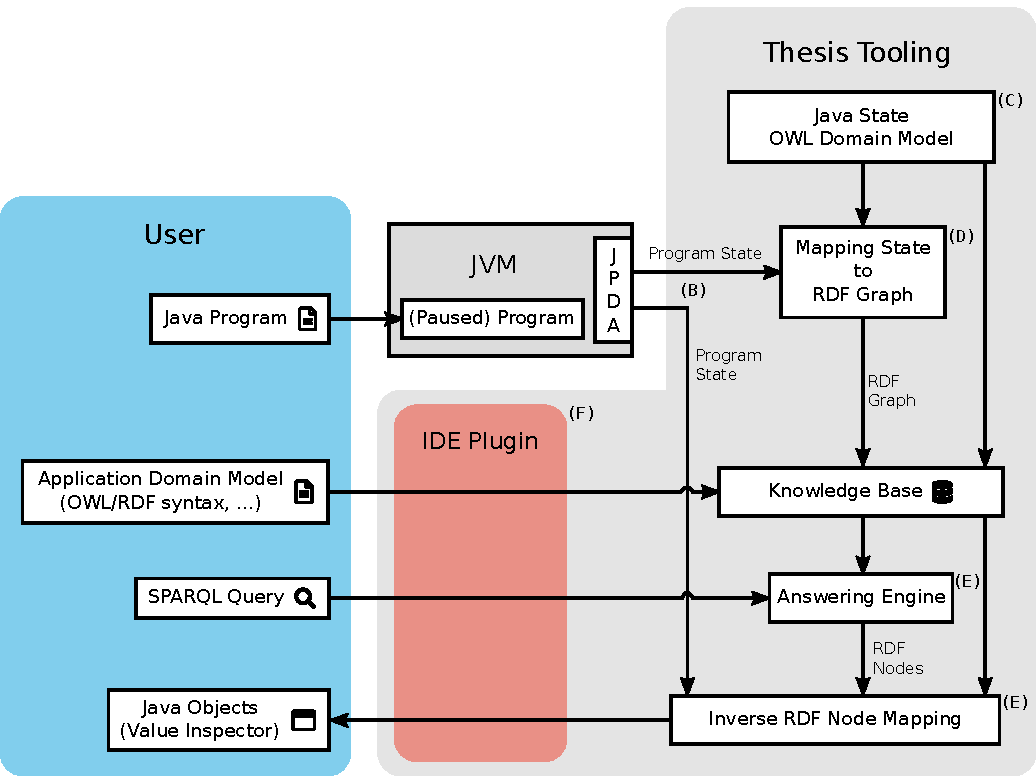
\includegraphics[width=0.8\linewidth]{gfx/workflow.pdf}
  \caption{%
    Informal illustration of a typical debugging workflow showcasing the
    different components of the tooling that is to be developed.
    %
    Where applicable, the identifying letter of a work package has been
    annotated to those components it is responsible for.
    %
    Icons by Font Awesome~\cite{fontawesome}, licensed under CC BY 4.0
    license~\cite{falicense}.
  }%
  \label{fig:workflow}
\end{figure}

\paragraph{List of packages}

\begin{description}
  \item[A: Familiarization with Semantic Web Technologies]
    The thesis project will need to integrate many established Semantic Web
    technologies.

    This includes\ldots
    \begin{description}[font=\normalfont]
      \item[The \emph{Resource Description Framework (RDF)}]
        %
        A language for describing structured information as triples.
        These triples relate subjects and objects via a predicate and can form
        an \emph{RDF graph}.

        As one part of the thesis, JVM program states will need to be mapped to
        RDF graphs. This way, the program state can be processed by other
        Semantic Web technologies.
        %
      \item[The \emph{SPARQL Protocol And RDF Query Language}] % TODO Example
        %
        A language which allows to query RDF graphs.
        In particular the thesis aims to allow users to inspect JVM states
        during debugging by issueing SPARQL queries.
        %
      \item[The \emph{Shapes Constraint Language (SHACL)}]
        %
        SHACL shapes allow to formulate constraints on RDF graphs.
        For example that certain resource types must have certain properties,
        the types of those properties, range constraints on the values of these
        properties etc.
        %
        Existing Semantic Web Frameworks like Apache Jena allow to automatically
        validate RDF data against those constraints.
        %
        SHACL Shapes have a potential use in a debugging scenario as they
        permit developers to verify that program states do not violate their
        expected format or to detect such violations.

        Thus, SHACL support may be implemented in addition to SPARQL query
        support.
        %
      \item[The \emph{Web Ontology Language OWL}]
        %
        With OWL, \emph{ontologies} can be formalized. That is, a description of
        a subject area, its concepts, their properties and relations.

        For example, as part of the thesis, an OWL domain model for Java program
        execution states will be developed.
        It shall describe the different entities and ideas of an (executed) Java
        program (classes, objects, methods, \ldots) and their relationships
        (e.g. objects are instances of classes).
        Such an OWL model is needed to give RDF graphs of programs semantics in
        the Java domain.
        This is similar to the OWL model for the SMOL language of
        \cite[Fig. 2]{kamburjan2021programming}.
        
        Furthermore, user-provided OWL classes can further infer application
        domain concepts from the Java OWL model. % TODO: Validation / conistency of this user provided model??
        I.e. users may define how classes and objects form a Simple Graph,
        its vertices and edges.
        %
      \item[The \emph{Apache Jena Java Framework for Semantic Web Applications}]
        %
        Apache Jena allows to leverage the aforementioned Semantic Web
        technologies (reading / writing RDF graphs, performing SPARQL queries,
        etc.).

        Usage of Apache Jena will accelerate this project as Semantic Web
        technologies do not need to be re-implemented.
        %
      \item[(...potentially more relevant technologies...)]
      % \item[HermiT] TODO
    \end{description}

    The Semantic Web and its technologies are a complex and rich topic.
    Thus, getting acquainted with these technologies and becoming able to use
    them is a critical component of this thesis.

    \textbf{This work package includes:}
    \begin{itemize}
      \item Getting familiar with the above Semantic Web technologies.
        That is, reading relevant introductory literature and experimenting with
        tooling.
        %
      \item Summarizing and explaining those Semantic Web concepts that are
        vital for understanding the thesis to the reader.
    \end{itemize}
    %
  \item[B: Pausing Java program execution \& Accessing JVM State]
    %
    A core goal of the thesis is to debug Java programs. For this, the developed
    tool must be able to halt the execution of a Java program and be able to
    inspect its state.

    Via the \emph{Java Debugger Architecture (JPDA)}~\cite{jpda}, and in
    particular its \emph{Java Debug Interface (JDI)} component one can
    \begin{itemize}
      \item set breakpoints
      \item step through a program
      \item inspect the program state
      \item \ldots
    \end{itemize}

    For example, the \lstinline|VirtualMachine| interface~\cite{VirtualMachine}
    of the JDI can list all \lstinline|ReferenceType|s, e.g. all classes, their
    fields and values etc.
    It also permits access to all threads, their \lstinline|StackFrame|s,
    variables and values.

    \textbf{This work package includes:}
    \begin{itemize}
      \item Getting familiar with the JPDA
      \item Implementing a proof-of-concept program capable of pausing other
        Java programs and extracting the most vital JVM state information
        (e.g. classes, methods, objects, \ldots)
    \end{itemize}
    %% Java Platform Debugger Architecture (JPDA)
    %
    % 3 Modules
    %
    % * JVM TI: JVM Tools Interface
    %   * Services a VM implementation must provide for debugging
    %
    % * JDWP: Java Debug Wire Protocol
    %   * Defines format / protocol of communication between process being debugged
    %     and debugger
    %
    % * JDI: Java Debug Interface
    %   * debugger must implement this set of interfaces
    %   * allows access to
    %     * VM state
    %     * debugged process variables
    %     * set breakpoints
    %     * stepping
    %     * watchpoints
    %
    %   * in particular the following can be retrieved
    %     * all reference types in a program, e.g. all classes, their methods, fields etc.
    %     * all threads, their stackframes, variables and values etc.
    %
    % https://docs.oracle.com/javase/7/docs/technotes/guides/jpda/
    % https://www.baeldung.com/java-debug-interface
    %
    %%
    %
  \item[C: An OWL model for Java program states]
    %
    As mentioned in work package (A) and before, an RDF graph must be
    extracted from a JVM state as provided by package (B).
    
    However, to be able to meaningfully construct such a graph, it must be
    given semantics in the domain of execution states of Java programs.

    Thus, a suitable OWL model of this domain must first be developed.
    There already exists work on ontologies for the knowledge domain of the Java
    Programming Language, e.g.~\cite{kouneli2012modeling,atzeni2017codeontology}.
    This work may be adapted to develop a new ontology suited for this thesis.
    A particular challenge is to develop the ontology such that it
    not only describes static source code, but also captures concepts of a Java
    program paused during execution.
    On the other hand, Java is a very rich language and describing every one of
    its features would not fit into the time constraints of this thesis.

    Thus, the developed OWL model should be restricted to a core set of features
    suitable to implementing the most basic semantic debugging features.

    \textbf{This work package includes:}
    \begin{itemize}
      \item Researching existing ontologies for the knowledge domain of the Java
        language. This includes identification of the methodology by which
        ontologies for object-oriented programming languages are created in
        general.
        %
      \item Determining the subset of core domain concepts relevant to this thesis.
        %
      \item Developing an ontology encompassing these core concepts.
        %
      \item Formalizing it in OWL.
    \end{itemize}
    %
  \item[D: Mapping Java program states to RDF knowledge graphs]
    %
    As outlined before, to apply any sort of Semantic Web tooling to the the
    state of a Java program, it must first be converted to an RDF graph, a
    format commonly understood by such tooling.

    More specifically, a map must be developed which maps Java program states
    to an \emph{ABox}. % TODO: Paper says TBox here, but this seems wrong...
    An \emph{ABox} is a notion from \emph{description logics} on which OWL is
    built.
    It is a collection of assertions describing to what concepts a
    certain object belongs and what roles and relationships they assume within
    a domain.

    It may for example describe, that a certain object belongs to a
    certain class. And it may say that that class has a specific field etc.
    Thus, the output of this mapping relies on the OWL domain model developed
    in work package (C).

    On the other hand, to properly define such a mapping, a formalization of
    the Java states retrieved through work package (B) may also be needed.
    There exist (partial) formalizations of the Java language, some of which
    explicitly model intermediate program states
    (e.g. \cite{feitosa2018formal,bogdanas2015kjava}).
    Some of these state models may suitable to be adapted for this thesis.

    Ultimately, a model of Java states must be worked out which...
    \begin{itemize}
      \item ...can preserve the high-level view of the program state provided by
        the JDI (see work package (B)).
        That is, a state model that is aware of stack frames, classes, fields etc.
        is more useful for constructing an RDF graph than a store of memory
        addresses and primitive values.
        %
      \item ...restricts itself to core concepts of Java.
        Capturing all Java features is outside the scope of this thesis.
        %
    \end{itemize}

    \textbf{This work package includes:}
    \begin{itemize}
      \item Research existing models of Java program states.
      \item Evaluate which features of such a model are essential to implement
        a mapping as described.
        %
      \item Develop a suitable model of Java program states.
        Implement subroutines to automatically extract instances of this model
        from the JDI.
        %
      \item Implement the mapping from program states to \emph{ABox}s
    \end{itemize}
    %
  \item[E: Query Answering Engine]
    A central feature of the debugger developed in this thesis is the ability to
    perform queries on the program state using SPARQL.
    Moreover, these queries should be able to ask about concepts from the Java
    ontology of work package (C), as well as ask about concepts from a
    user-provided application domain.
    %TODO Example

    To realize this feature, an \emph{answering engine} must be implemented.
    An answering engine is a function which takes a knowledge base as well as a
    query as input, and yields all objects and entities in the knowledge base
    which satisfy the query.

    In the context of this thesis, the knowledge base consists of up to three
    components:
    \begin{itemize}
      \item The set of OWL axioms defining the Java state ontology
        (work package (C)).
        %
      \item Optionally, a set of user-provided OWL axioms describing the
        application domain.
        %
      \item The RDF graph resulting form work package (D)
    \end{itemize}

    The query shall be provided in the SPARQL language.
    This allows us to utilize the existing ARQ query engine~\cite{arq} of Apache
    Jena which can answer the SPARQL query given the above input information.

    The query engine will return nodes from the RDF graph satisfying the
    query.
    However, just the RDF representation of those nodes may not be sufficient
    to effectively debug an application since the user may need to inspect the
    corresponding Java objects or constructs from which the RDF nodes
    have been created.
    Hence, part of this work package is also to extend the mapping of package
    D to be (partially) reversible.
    That is, it should be at least possible for RDF nodes representing Java
    objects to retrieve those objects from the JVM state.
    %%% TODO Think about this
    %% Note that not every concept that can be queried may correspond to a single
    %% class. For example a user-defined application domain may define a concept
    %% as the union of two classes, thus 
    % TODO Example

    \textbf{This work package includes:}
    \begin{itemize}
      \item Combine the results of the previous work packages and Apache Jena
        to implement an answering engine as described.
        %
      \item Extend the mapping of work package (D) to be (partially)
        reversible as described.
    \end{itemize}
    %
  \item[F: IDE Integration]
    Integrated Development Environments (IDEs) for Java like
    \emph{IntelliJ IDEA}~\cite{idea} already include
    \enquote{traditional debuggers} which allow to directly inspect objects and
    values in a paused program state.

    This thesis aims to provide a new debugger for a mainstream programming
    language. In this spirit, it should also integrate well with mainstream
    tooling of that language and be readily available for use in common IDEs.

    For this work package, the thesis tooling as described by the previous
    work packages shall be integrated into an IDE as a plugin.
    More specifically, the plugin to be developed shall integrate a
    \emph{Read-Evaluate-Print-Loop (REPL)} into the UI of the IDE.
    Also, it should allow users to supply their own application domain
    definitions, e.g. as files defining an ontology in RDF/OWL syntax.

    The REPL will be available during debugging when execution is paused
    via breakpoint etc.
    It shall allow the user to input a SPARQL query.
    If the user inputs a query, the current state of the paused program shall
    be mapped to an RDF graph using the results from package (D).
    Then, the query and graph are to be processed by the answering engine of
    work package (E).
    Using the reverse mapping of work package (E), all Java objects
    corresponding to the results of the answering engine shall be retrieved.

    These objects shall then be displayed as a manually inspectable tree view,
    similar to those known from the value inspectors of traditional debuggers.
    % TODO: Example

    Optionally, a visualization or inspection tool for the RDF graph itself may
    also be implemented.

    Note, that the integration of the plugin with the existing debugging system of an IDE
    might pose a particular technical challenge since it may not be possible to
    attach multiple JPDA debuggers to the same Java process.
    That is, the debugger built into the IDE and the debugger from work package (B).
    % Link?

    If it is not possible to attach multiple debuggers, there are two possible
    ways to resolve this problem:
    \begin{enumerate}
      \item Either the plugin must not be integrated with the IDE debugger and
        act as a completely separate feature.
        This, however, may lessen the user-experience since users may not be
        able to seamlessly switch between traditional and semantic debugging
        without restarting the program to be debugged.
        %
      \item Or, the implementation of work package (B) must be rewritten not
        to directly leverage the JPDA but to extract all necessary information
        from the IDE debugger.

        This approach comes with two disadvantages. For one, the thesis tooling
        will then be tightly coupled to the API of a particular IDE.
        Secondly, the interface of the built-in IDE debugger may not be
        well-documented.
        For instance, the documentation of the
        \emph{IntelliJ Platform Plugin SDK}~\cite{pluginsdk} does not directly
        document the debugger. There is only a link to the relevant source code
        (\lstinline|XDebuggerManager|) in the list of extension points.
    \end{enumerate}
    The drawbacks of either approach must be evaluated and one of them be
    implemented.

    \textbf{This work package includes:}
    \begin{itemize}
      \item Learn about the plugin API of a popular Java IDE, e.g.
        IntelliJ Idea.
        %
      \item Implement the UI as described.
        %
      \item Evaluate the possible means of integrating the semantic debugger
        with the existing debugger interface of the IDE as discussed above.
        %
      \item Integrate the results of the previous work packages into the
        plugin as described.
        %
    \end{itemize}
    %
  \item[G: Case Study -- Debugging Example]
    An illustrative example shall be worked out that demonstrates the
    capabilities of the tooling that is developed in this thesis.

    That is, an easy to understand but not entirely trivial Java application
    must be written. Ideally, the implementation should slightly differ from the
    application domain and allow to represent invalid states.

    For example, \citeauthor{kamburjan2021programming} provide an implementation
    of the \emph{2-3 tree} data structure in \cite{kamburjan2021programming}
    for the SMOL language. It syntactically permits the instantiation of invalid
    tree nodes. This is due to efficiency optimizations
    of the implementation.
    \Citeauthor{kamburjan2021programming} then argue that their implementation
    of semantic debugging tooling for SMOL can help to debug such violations. 

    Similarly, the example application to be developed for this work package
    should also be faulty and produce a state violating the concepts of the
    application domain.
    Then, in a case study, it shall be demonstrated how the tooling from the
    previous work packages can be applied to fix the fault
    (e.g. querying the RDF graph of a faulty state etc.).

    \textbf{This work package includes:}
    \begin{itemize}
      \item Implement a suitable example of a faulty Java application as
        described.
        %
      \item Document the debugging process in a case study.
        %
    \end{itemize}
    %
  \item[H: Case Study -- Performance]
    % Microbenchmarks, scalable over N?
    An example application shall be implemented which features a data structure 
    of scalable size $n$.
    If the application from work package (G) already includes such a data
    structure, it may be reused.

    Then, a case study evaluating the performance of the thesis tooling shall be
    conducted for increasing $n$.
    Here, multiple different metrics may be relevant to assess the performance:
    \begin{itemize}
        \item Execution time and memory requirements for computing the RDF graph
          from a Java state.
          %
        \item Execution time and memory requirements for running SPARQL queries
          of differing complexity on the RDF graphs.
          %
        \item Execution time and memory requirements for computing increasingly
          complex inferences via the Apache Jena reasoner on the generated RDF
          graphs.
          %
        \item \ldots
    \end{itemize}

    \textbf{This work package includes:}
    \begin{itemize}
      \item A Java implementation of a data structure scalable in size as
        described. (If it can not be adapted from work package (G).)
        %
      \item Developing a suitable formalization of the application domain. % TODO Is application domain the right word here?
        %
      \item Developing suitable SPARQL queries and inferences for the Jena
        reasoner for a performance evaluation.
        %
      \item Conducting an performance evaluation as described.
        %
    \end{itemize}
    %
    %%
    % TODO: Optionals!
    %%
\end{description}

%% Packages
% * Understanding Semantic Web topics
% * mapping program states to knowledge graphs of internal domain
%   * Mapping JVM states to knowledge graph (RDF)
%     * JVM is huge, maybe do mapping of subset of JVM features first
%     * ...and extend later, if there is time
% * Answering Engine
%   * mapping knowledge base + query to set of answers
%   * Apache verwenden
% * Integration into an IDE
%   * IntelliJ Plugin?
%   * Support for loading user-specified domain models (application domain) in OWL DL (description logic)
%     * syntax support?
%     * validation?
%     * visualization of model?
%   * REPL (Read-evaluate-print-loop) for Queries
%     * Query state with SPARQL
%     * Validate state against SHACL
%       * if we support application domain definitions, do we need SHACL?
%     * Retrieve members of OWL classes
%     * Input: Text
%       * validation + debugging of queries?
%     * Output:
%       * Objects matching query
%       * (Local) Visualization?
%   * there is integration of SHACL for eclipse already...
% * Evaluation
%   * Performance?
%     * Skalierbarkeit
%       * skalieren über n
%       * kann es auf großen Datenmengen laufen
%   * Reasoner: Inferenzen von Relationstuplen
%     * Problem: Macht Ausführung deutlich langsamer
%     * Wie skaliert dies bei immer komplexeren Abfragen?
%     * Entweder Jena Reasoner (bevorzugt) / oder Hermit
%   * größeres Beispiel
%   * User-study?
%     * wahrscheinlich eher nicht
%     * optionales Paket
% * Optimization
%   * do not compute complete knowledge graph eagerly
%   * instead, lazily compute only required parts
%   * virtualisierung: Optional
% * textual artifact
%   * description of implementation
%   * related work discussion
%   * case studies
%   * Wartbarkeit + Erweiterbarkeit
%     * zentral
%     * sollte dokumentiert sein
%   * enable semantic state access
%     * Reflection also part of this thesis?
%       * nicht geplant
% * Computational Semantic State Access?
%   * i.e. deriving implicit information (e.g. area from height and width of a rectangle)
%   * integrate it directly into Java classes (e.g. marking methods with annotations)
%     or external extension methods?
%   * nicht geplant
%
% * Theoretischer Anteil
%   * Tatsächliche Implementierung (Bytecode) sehr unterschiedlich zu Domänenmodell
%   * Noch unklar, Problem wird während Implementierung auftauchen
%   * Anwendung auf echte Programmiersprache wissenschaftlich genug
%%

\section{Time Schedule}%
\label{sec:time_schedule}

\subsection{Available Time}
The M. Sc. Computer Science course at TU darmstadt allocates 30 credit points
for the master thesis and it must be written within 26 weeks.
At TU Darmstadt, a credit point translates to roughly 30 hours of work.

Hence, this thesis must be realized within
$30\text{CP} \cdot 30 \frac{\text{h}}{\text{CP}} = 900 \text{h}$ of work.

Therefore, when assuming an even distribution of the work, this corresponds to
about $900\text{h} / 26\text{w} \approx 34.6$ hours of work per week.

\subsection{Dependencies}
The work packages of \cref{sec:work_packages} partially depend on each
other. These dependencies also dictate the order in which they can be
implemented. The following diagram depicts those dependencies:

\begin{center}
  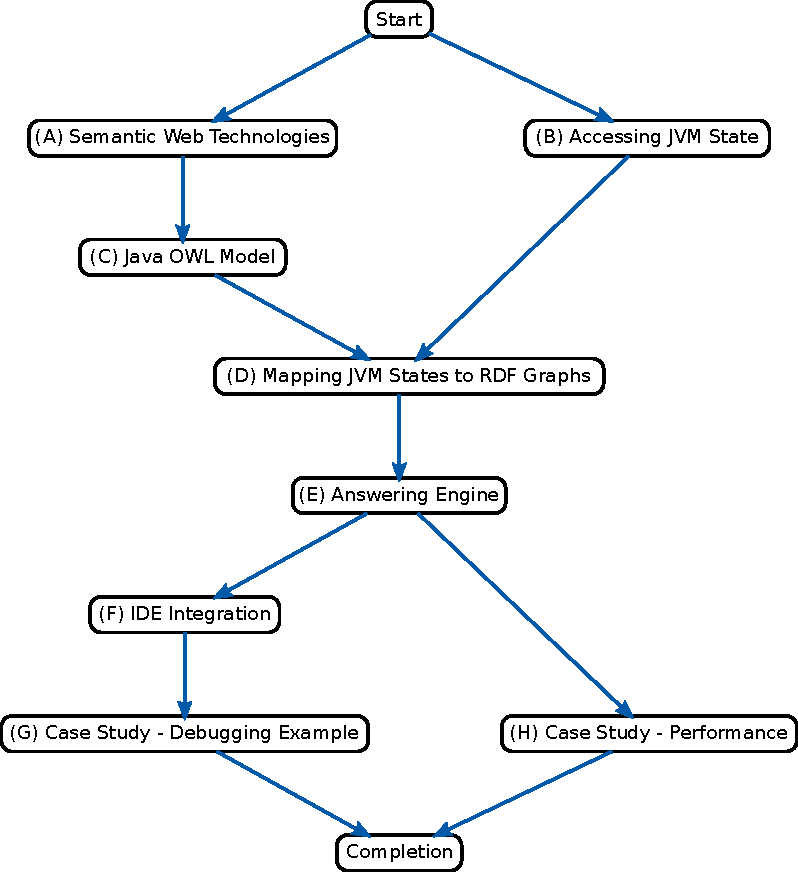
\includegraphics[width=0.6\linewidth]{gfx/dependencies.pdf}
\end{center}

Based on this system of dependencies, the following order has been decided for
implementing the work packages:

\begin{enumerate}
  \item (A) Semantic Web Technologies
  \item (B) Accessing JVM State
  \item (C) Java OWL Model
  \item (D) Mapping JVM States to RDF Graphs
  \item (E) Answering Engine
  \item (F) IDE Integration
  \item (G) Case Study -- Debugging Example
  \item (H) Case Study -- Performance
\end{enumerate}

Even though (C) does not necessarily depend on (B), (B) should be implemented
beforehand: The knowledge about the JVM state data accessible through the JPDA
might be useful for developing an appropriate Java State OWL model.

Since the example of case study (G) may be reusable for the case study (H), (G)
should also be realized before (H).

\subsection{Schedule}

Available time: 26 weeks. The following is an approximate schedule for
implementing the work packages:
\bigskip

\begin{center}
  \begin{tabular}{llll}
    \toprule
    Work Package & Alotted Time & Due Date\\
    \midrule
    (A) Semantic Web Technologies        & 2 weeks & 2021-11-14 \\
    (B) Accessing JVM State              & 2 weeks & 2021-11-28 \\ % Seminar presentation
    (C) Java OWL Model                   & 5 weeks & 2022-01-02 \\ 
    (D) Mapping JVM States to RDF Graphs & 5 weeks & 2022-02-06 \\ % intermediate
    (E) Answering Engine                 & 4 weeks & 2022-03-06 \\ % exam, seminar paper
    (F) IDE Integration                  & 2 weeks & 2022-03-20 \\
    (G) Case Study -- Debugging Example  & 2 weeks & 2022-04-03 \\
    (H) Case Study -- Performance        & 2 weeks & 2022-04-17 \\
    Thesis Finalization                  & 2 weeks & 2022-05-01 \\
    \bottomrule
  \end{tabular}
\end{center}

\bigskip
\noindent
Parallel to the master thesis, some additional workloads have to be taken
into account: A seminar course, an intermediate presentation on the thesis
results, and one exam (no course attached):

\begin{itemize}
  \item Seminar Presentation: Likely around 1st December.
    This is around 4 weeks after the start of the thesis.
    %
  \item Intermediate Thesis Presentation. After around half of the alotted time.
    Therefore around 13 weeks after the start of the thesis which is at the
    start of January.
    %
  \item Exam: Likely around mid-February which is around 15 weeks after the
    start of the thesis.
    %
  \item Seminar Paper Submission: Around 20th February.
    This is around 16 weeks after the start of the thesis.
    %
\end{itemize}
%
With this additional workload in mind, the time allotted has been slightly
increased for those work packages to be implemented at the same time as the
above dates.

\printbibliography

\end{document}
